\documentclass[14pt, a4paper]{article}
\usepackage{float}
\usepackage{graphicx}
\usepackage[utf8]{inputenc}
\usepackage[margin=1in]{geometry}

\DeclareGraphicsExtensions{.png}

\begin{document}

%\title and intnro
\begin{titlepage}
	\begin{center}
		
		\begin{figure}[t]
			\centerline{
			
\includegraphics[width=450px]{./Graphics/KPTH_Logo.png}}
		\end{figure}		
		
		\textbf{\LARGE Gynaecological Patient Information
		management System:}
		
		\vspace{1 cm}
	    \textbf{\LARGE \\User Manual}
		
		\vspace{1 cm}
		\LARGE{\textbf{Team Pentec: }}
		

		\begin{flushright} \large
			
			Ruth Ojo 12042804\newline
			Liz Joseph 10075268\newline
			Trevor Austin 11310856\newline
			Maria Qumayo 29461775\newline
			Lindelo Mapumulo 12002862\newline
		\end{flushright}
		
				\vspace{1 cm}
				\centering
				
\includegraphics[width=150px]{./Graphics/Pentec_Logo.png}

		
		{\LARGE Version 1.4} 
		\\
		{\large \today}		
		
		
	\end{center}
\end{titlepage}


\begin{abstract}
\Large
This document is the Software User Manual (SUM) for the Patient Information Management System project and was made according to the software engineering standard described in the tender proposal provided by Professor Snyman. The Software User Manual (SUM) instructs how to install and use the
Patient Information Management System software. This project is part of the Software Engineering Project course (COS301) at the University of Pretoria.\\
\end{abstract}

\newpage

%\table of content
\tableofcontents
\newpage

\section{Introduction}


\subsection{Change Log}
Document Title: Software User Manual\\
Version: 0.1.0\\
Document Status: conditionally approved\\
Version Date Author(s) Summary\\
0.0.1 29-05-2015 Pentec Document creation\\


\subsection{Intended readership}
This document covers the use for the following users of the PIMS system:\\
\begin{description}
\item the system administrator
\item the project administrators
\item the medical staff
\item the usability test subjects
\end{description}

\subsection{Applicability}
This Software User Manual (SUM) applies to the PIMS software, version 0.1.\\


\subsection{Purpose}
The purpose of the SUM is to assist the user in installing and using the PIMS software.\\

	
\subsection{How to use this document}
\begin{description}
\item How it is to be used:
\item[$\bullet$] Title page - System name and the names and/or affiliation of all stakeholders.
\item[$\bullet$] Introduction - Introduction to the System
\item[$\bullet$] Overview - Purpose of the system
\item[$\bullet$] Configuration - Configuration used by the system
\item[$\bullet$] Installation - Detailed description of where to find the software and how to install it.
\item[$\bullet$] Getting Starting - Walk through of the system
\item[$\bullet$] Using the System - Description of the systems functions
\item[$\bullet$] Troubleshooting - Procedures to take in case of errors
\end{description}

	
\subsubsection{Problem Reporting}
Since the Pentec team will be dissolved after completion of the PIMS project, the
issue of problem reporting is left to the Administrator, Professor Snyman.\\
	
	
\newpage

\section{Overview}
The purpose of this software is to be used by doctors and medical staff. It allows the administrative users to electronically fill in medical forms and be able to query for statistics for those forms and eventually receive a prediction that could assist in the functionality of the Kalafong Hospital. Regular users are allowed to fill in medical forms.
\\

\newpage

\section{Configuration}
\subsection{System Configuration}
\subsubsection{Basic System Structure}
The current system that is in place makes use of a Node.js server that interacts with any web client. The server is hosted through a PaaS named Heroku. The system delivers compiled jade files to the users that are stylized using CSS. The jade files are controlled and animated by Javascript and jQuery. The node.js server accesses MongoDB database hosted on the DaaS, mongolab. This is illustrated below:
\begin{figure}[h!]
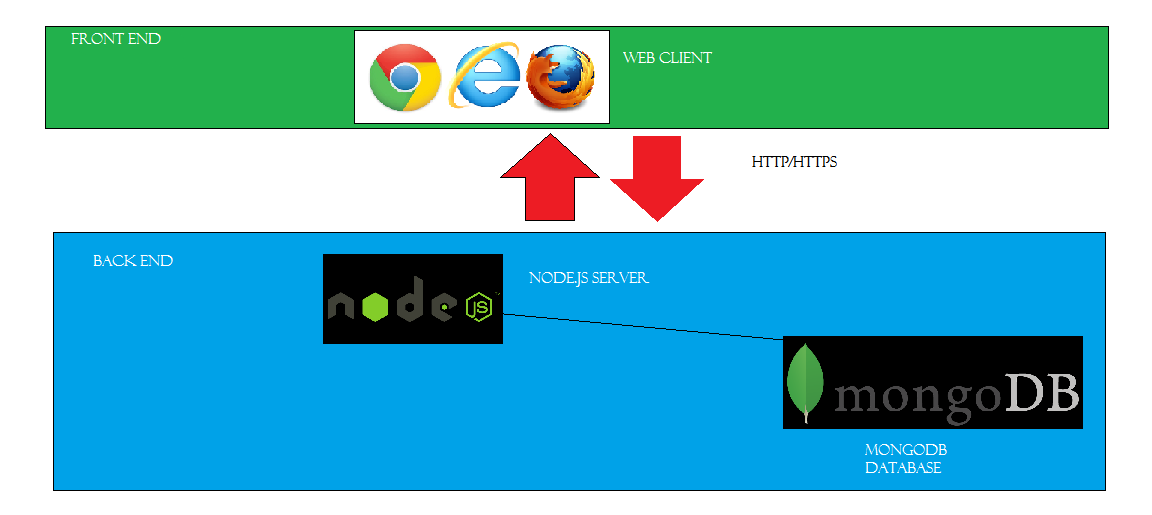
\includegraphics[width=1.0\textwidth]{Graphics/Screenshots/infrastructure}
\end{figure}
\newpage
\subsubsection{Node.js Architecture}
Node.js is an asynchronous langauge and its basic client-server communication is illlustrated below:
\begin{figure}[h!]
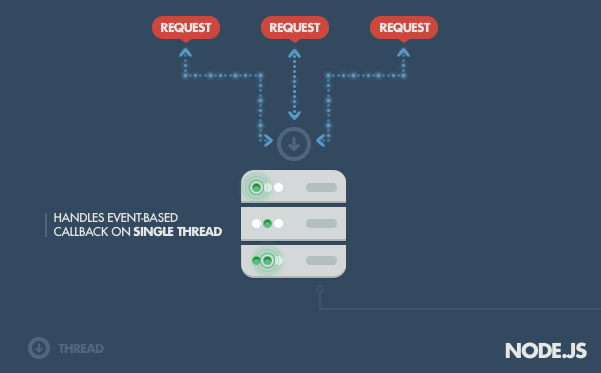
\includegraphics[width=1.0\textwidth]{Graphics/Screenshots/nodejsinfrastructure}
\end{figure}
\subsubsection{Communication Protocols Used}
This is the current list of all communication protocols used by PIMS:
\begin{itemize}
	\item HTTP/HTTPS
	\item SMTP
\end{itemize}
\newpage

\newpage

\section{Installation}
\subsection{Running the Software}
\subsubsection{Risks}
You cannot log into the website without javascript enabled. Recapture doesn't work without javascript enabled.
Please follow the instructions below if the recapture box does not appear.

\begin{enumerate}
  \item Website page
  \begin{enumerate}
  \item Establish an internet connection
  \item Search for website in web browser
 \item Steps to enable javascript in your chosen browser
    
  \item[$\bullet$] Google Chrome browser
    \begin{enumerate}
       \item Click the menu bar at the top right hand corner of your web browser
       \begin{figure}[H]
       \centerline{\fbox{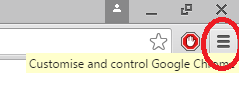
\includegraphics[width=0.3\textwidth]{Graphics/Installation/step1C}}}
		\caption{Menu}
      \end{figure}
       \item Select the settings option
       \begin{figure}[H]
         \centerline{\fbox{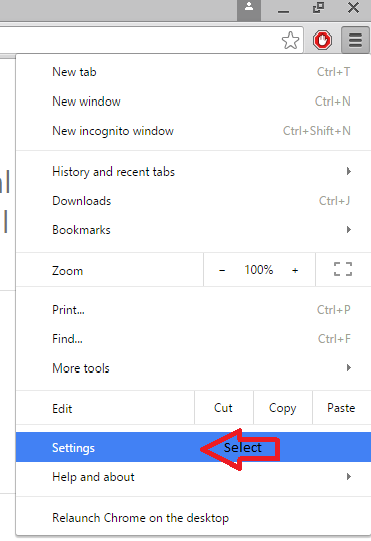
\includegraphics[width=0.3\textwidth]{Graphics/Installation/step2C}}}
		\caption{Settings}
      \end{figure}
       \item Scroll down to the bottom of the page and click on 'Show advanced settings'
       \begin{figure}[H]
         \centerline{\fbox{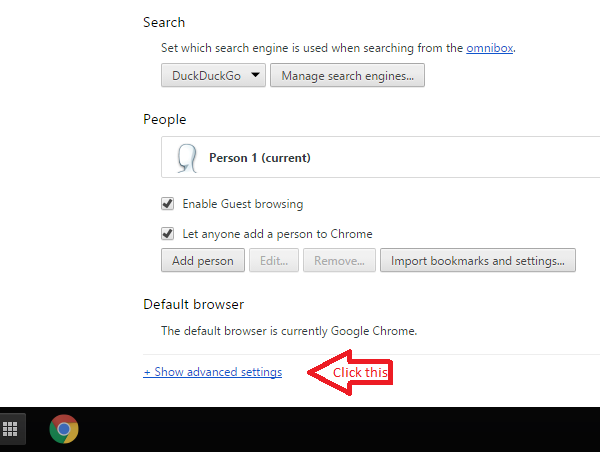
\includegraphics[width=0.4\textwidth]{Graphics/Installation/step3C}}}
		\caption{Advanced Settings}
      \end{figure}
       \item Scroll down to the Privacy Menu and click on the button 'Content settings..'
       \begin{figure}[H]
        \centerline{\fbox{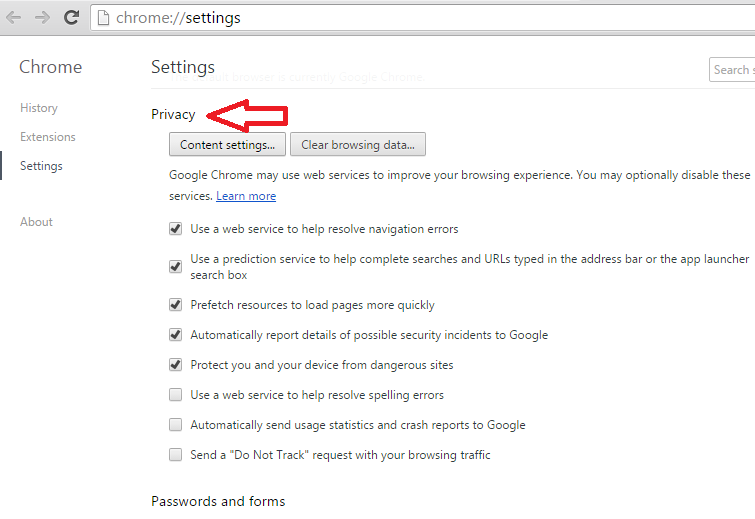
\includegraphics[width=0.5\textwidth]{Graphics/Installation/step4C}}}
		\caption{Content Setting}
      \end{figure}
       \item Scroll down to the Javascript Menu and select 'Allow all sites to run Javascript(Recommended)'
       \begin{figure}[H]
       \centerline{\fbox{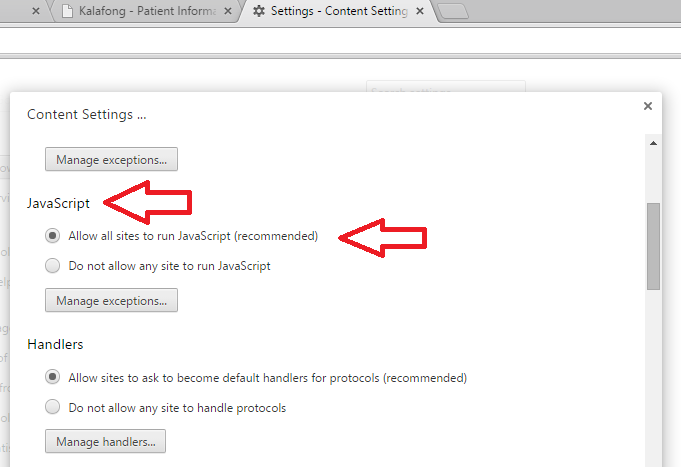
\includegraphics[width=0.4\textwidth]{Graphics/Installation/step5C}}}
		\caption{Enable}
      \end{figure}
       \item Click finished
     \end{enumerate}

  
\item[$\bullet$]  Internet Explorer browser
\begin{enumerate}
       \item Select the Gear in the upper-right corner of the screen or the 'Tools' menu if you have the menu bar enabled, then select 'Internet Options'.\\
        \begin{figure}[H]
       \centerline{\fbox{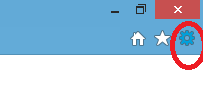
\includegraphics[width=0.4\textwidth]{Graphics/Installation/step1}}}
		\caption{Settings}
      \end{figure}
  \begin{figure}[H]
       \centerline{\fbox{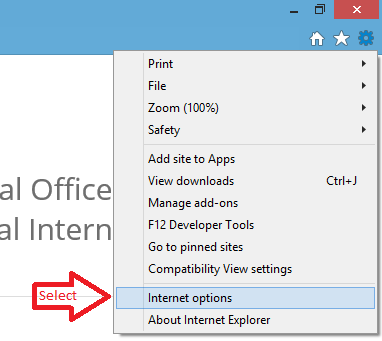
\includegraphics[width=0.4\textwidth]{Graphics/Installation/step2}}}
		\caption{Internet options}
      \end{figure}      
      
       \item Select 'Security' > 'Internet' > 'Custom level'
       \begin{figure}[H]
       \centerline{\fbox{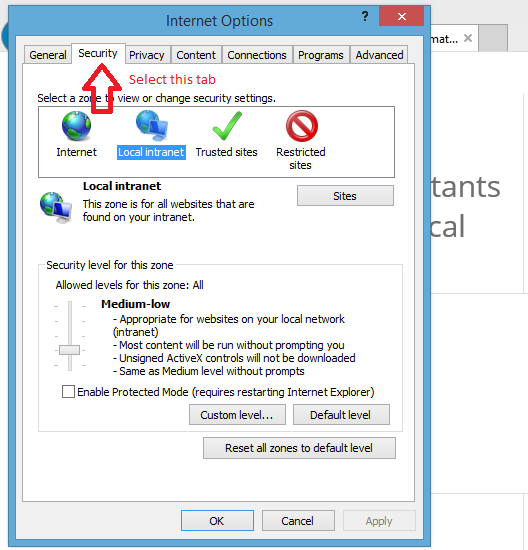
\includegraphics[width=0.4\textwidth]{Graphics/Installation/step3}}}
		\caption{Enable}
      \end{figure}
       \item Scroll down to 'Scripting' and select the radio button to 'Enable' or 'Disable' it. 
       \begin{figure}[H]
       \centerline{\fbox{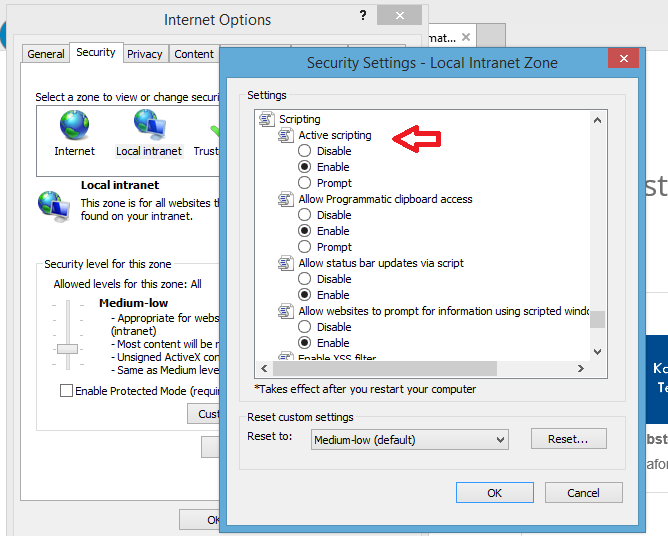
\includegraphics[width=0.5\textwidth]{Graphics/Installation/step4}}}
		\caption{Enable}
      \end{figure}
       \item You may also opt for IE11 to 'Prompt' you to allow scripts to run.
       \item Select 'OK', then 'OK' again.
     \end{enumerate}

  
    \item[$\bullet$]  Firefox browser
    \begin{enumerate}
   
       \item In Firefox's address bar, type about:config and press Enter.
       \item Click I'll be careful, I promise! button.
     \begin{figure}[H]
       \centerline{\fbox{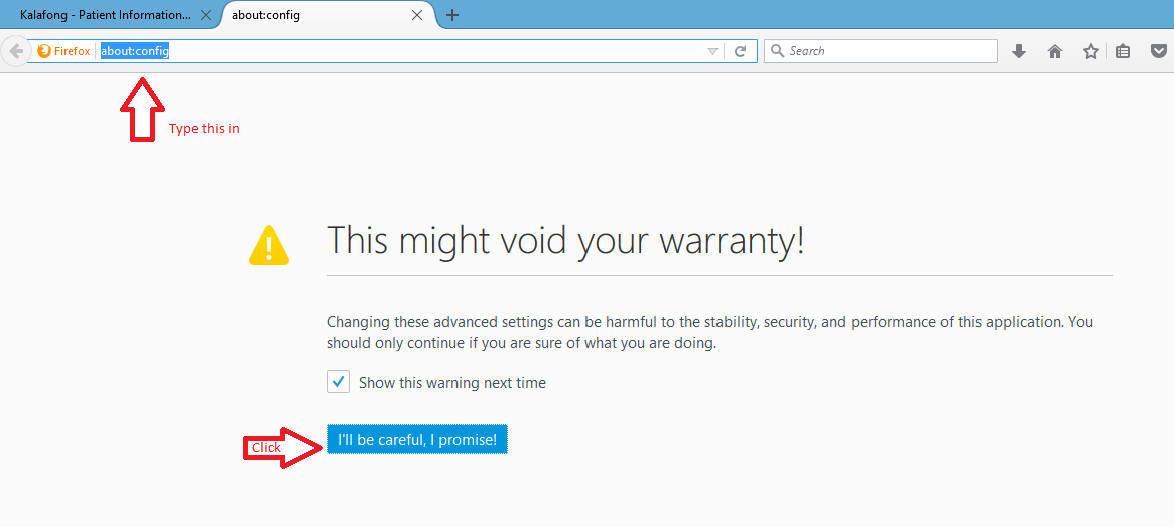
\includegraphics[width=0.4\textwidth]{Graphics/Installation/step1FF}}}
		\caption{Enable}
      \end{figure}       
       
       \item In the search bar, search for javascript.enabled.
     \begin{figure}[H]
       \centerline{\fbox{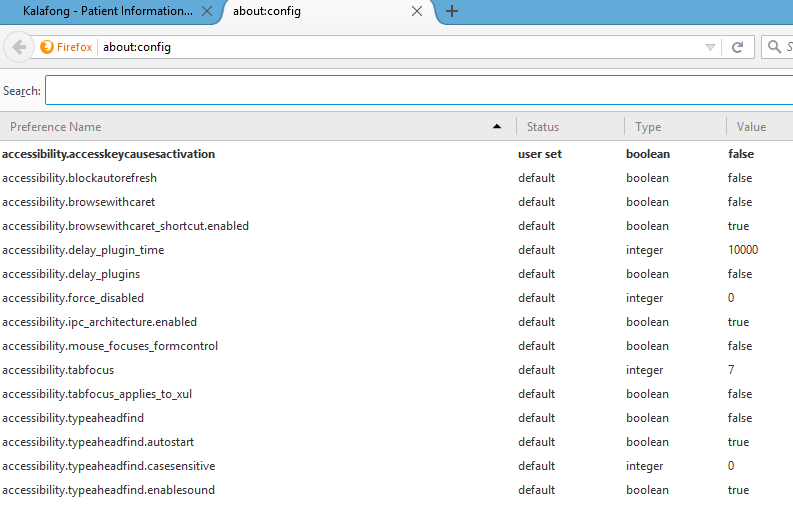
\includegraphics[width=0.5\textwidth]{Graphics/Installation/step2FF}}}
		\caption{Enable}
      \end{figure}         
       
       \item Double click on the row of preference named javascript.enabled to change the value to False. ...
       \begin{figure}[H]
       \centerline{\fbox{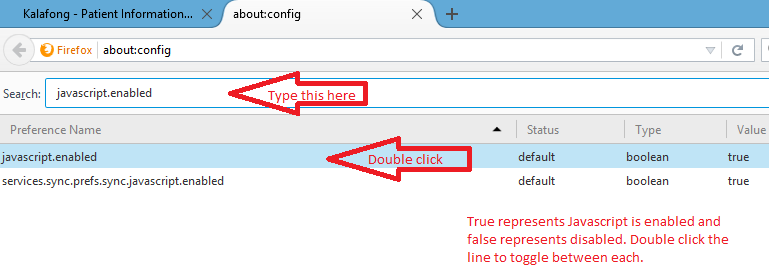
\includegraphics[width=0.5\textwidth]{Graphics/Installation/step3FF}}}
		\caption{Enable}
      \end{figure}   
      
       \item JavaScript is now disabled.
     \end{enumerate}

    \item Log into PIMS system with given authentication codes
  \end{enumerate}
 
\end{enumerate}


\subsubsection{How to register}
Users cannot register for the website they have to be given permission and login details to access the site by Admin(Dr Snyman).

\subsection{Shutting down the website}
Contact your service provider(hosting site) to pull down the software
\newpage



\section{Getting Started}
\subsection{Systems Procedure Order}
	This section describes a brief overview of how a user can access the system; it shows perspectives from an administrative user as well as normal users. The sections that are discussed can be found in more detail in the next section.
\subsection{Splash Page}
	\begin{figure}[H]
		\fbox{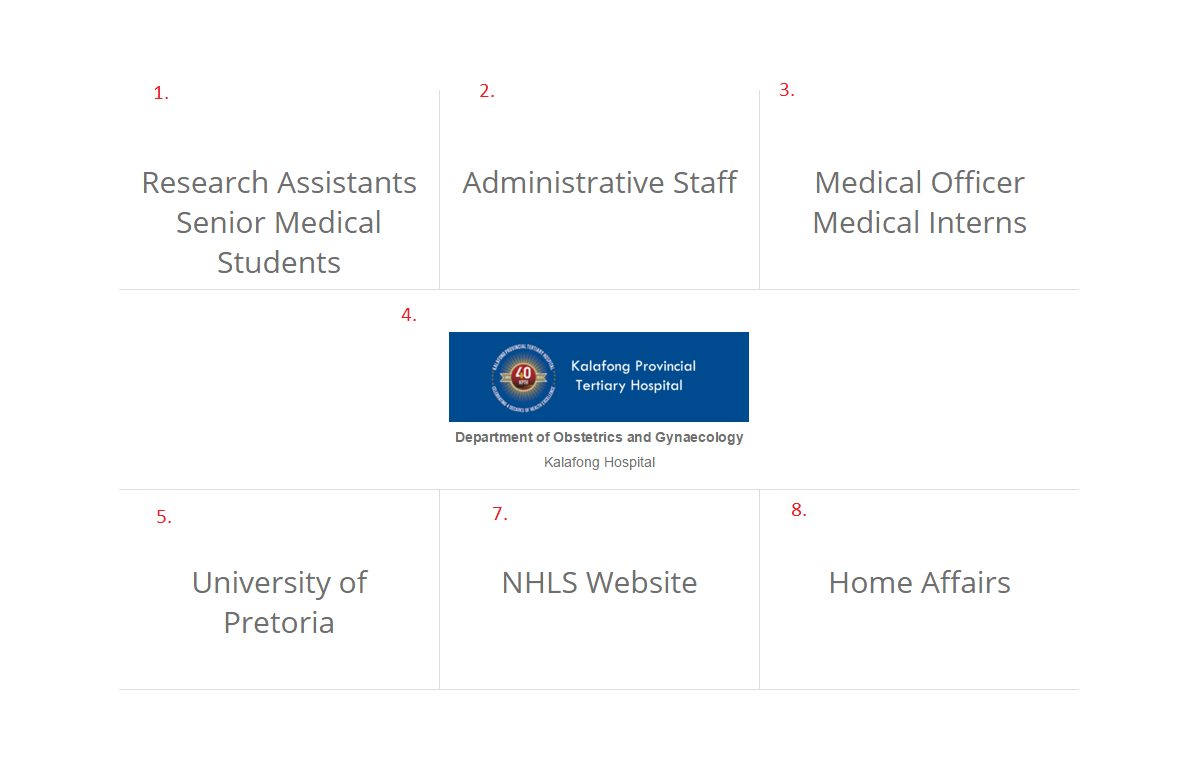
\includegraphics[width=1.0\textwidth]{Graphics/Screenshots/splash}}
		\caption{The splash page.}
		\label{fig:splash1}
	\end{figure}
	\subsubsection{Description}
		This section links users to different pages that they can access. A more detailed description of each component can be found below.
	\subsubsection{Detailed Component Description}
		\begin{enumerate}
			\item \textbf{Research Assistants \& Senior Medical Students Link:} This is a link that will direct the user to a customized login page for research assistants and senior medical students.
			\item \textbf{Administrative Staff Link:} This is a link that will direct the user to a customized login page for administrative staff.
			\item \textbf{Medical Officer \& Medical Interns Link:} This is a link that will direct the user to a customized login page for medical officers and medical interns.
			\item \textbf{Kalafong Hospital Link:} This link directly links users to the official University of Pretoria Kalafong hospital page.
			\item \textbf{University of Pretoria Link: } This link directly links users to the official university of Pretoria page.
			\item \textbf{National Health Laboratory Service Link:} This is a link that will direct users to NHLS website.
			\item \textbf{Home Affairs Link:} This is a link that will direct users to the home affairs website in order to allow users to check their life status.
		\end{enumerate}
	\subsubsection{Accessing user login}
		\begin{enumerate}
			\item Select the link that is relative to user's login. E.g. Research Assistants should click the Research Assistants \& Senior Medical Students link.
			\item More information on the login page in the login tutorial section\ldots
		\end{enumerate}
\subsection{Login}
	\begin{figure}[H]
		\fbox{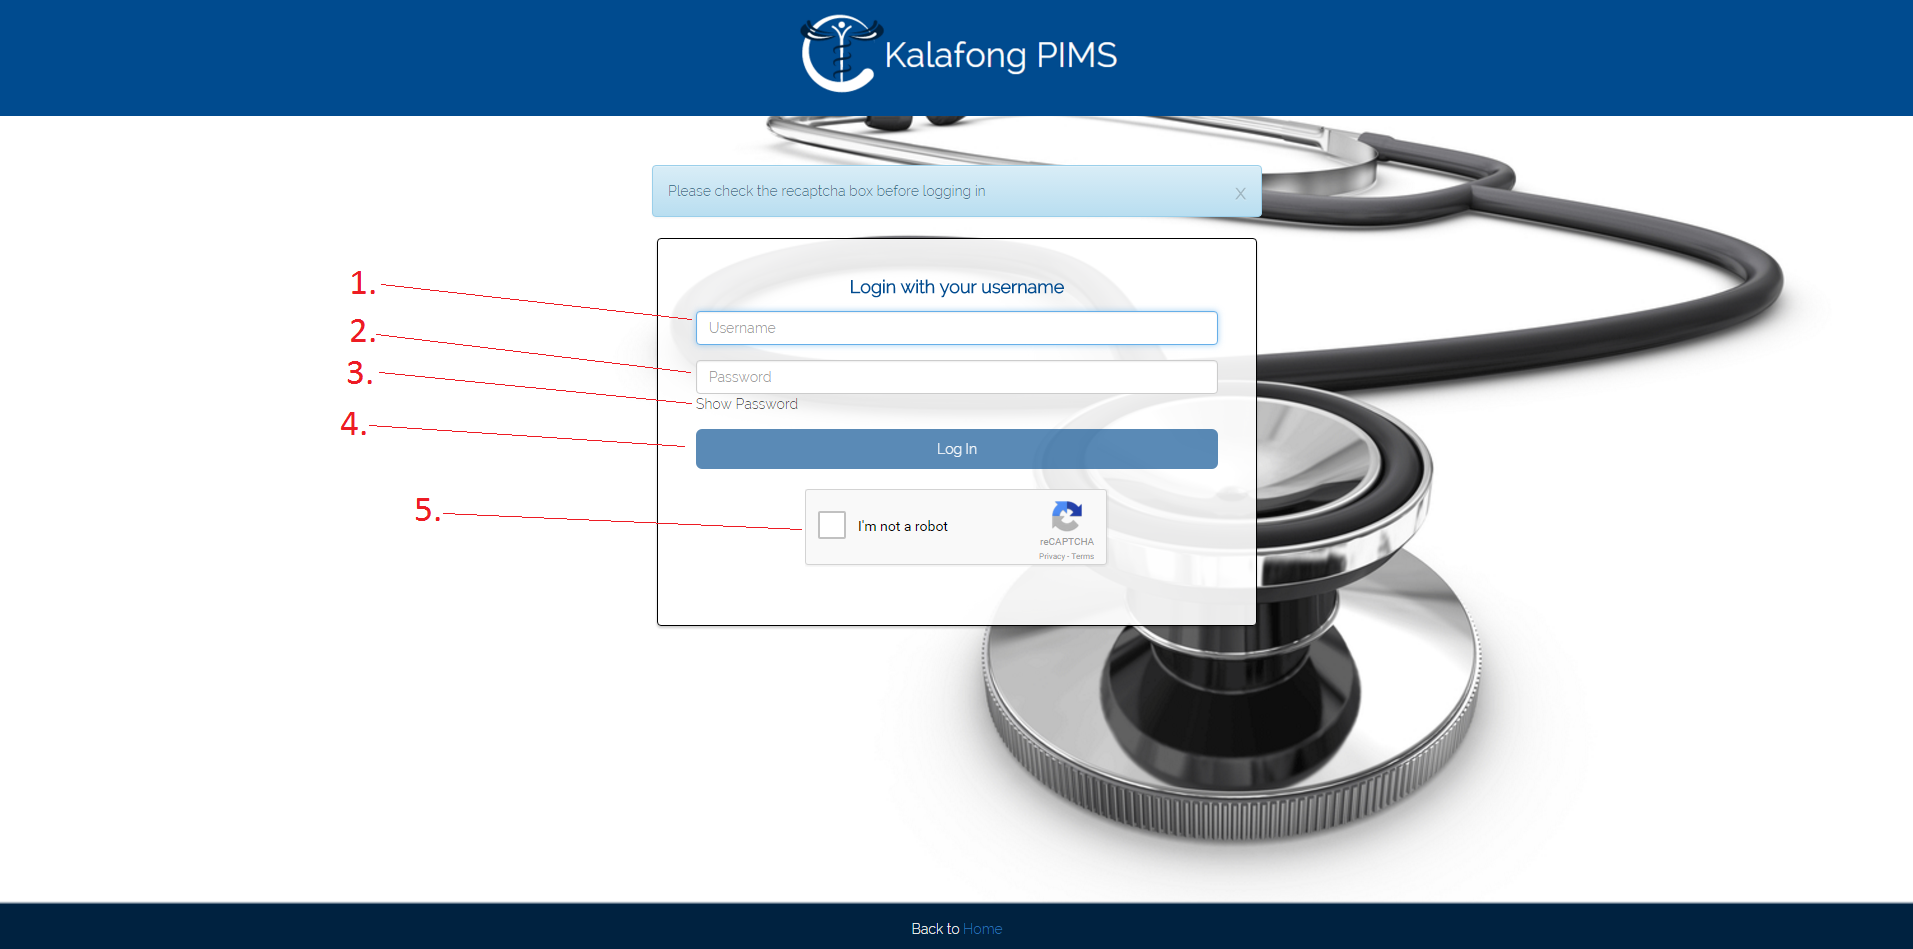
\includegraphics[width=1.0\textwidth]{Graphics/Screenshots/loginMain}}
		\caption{The login page.}
		\label{fig:login1}
	\end{figure}
	\subsubsection{Description}
		This is the login page that all users must access before being able to access the main web page. Users must fill in their credentials and pass a security check to be able to access this page. More detailed information can be found below.
	\subsubsection{Detailed Component Description}
		\begin{enumerate}
			\item \textbf{Username Input Box:} This is the input box in which users will enter in their username.
			\item \textbf{Password Input Box:} This is the input box in which users will enter in their password.
			\item \textbf{Show Password Button:} This button allows users to check their password text. Clicking this button will toggle between whether the password is shown or not.
			\item \textbf{Login Button:} This is the button the users will click once they have filled in their information and passed the security check. This will link them to their relative my space page.
			\item \textbf{Recaptcha: } This is the security check that is put in place. More information on how to use it is placed within the \textit{"How to Login"} section.
		\end{enumerate}
	\subsubsection{How to login}
		\begin{enumerate}
			\item Fill in username input box and confirm it is correct. NOTE: If the user login page does not look like the above do not panic. There are different themes for each user type. The other themes can be found at the bottom of the login section in figure \ref{fig:login2}.
			\item Fill in password input box and confirm it is correct. The user can confirm the password is correct using the show password button.
			\item Complete the security check for the recaptcha by clicking on the recaptcha checkbox.
			\item If multiple logins have been made in succession, a user may be prompted to select certain images related to a theme. For example, below (Figure \ref{fig:recaptcha1}) the recaptcha is asking the user to select all images with street signs.
			\begin{figure}[H]
				\centerline{\fbox{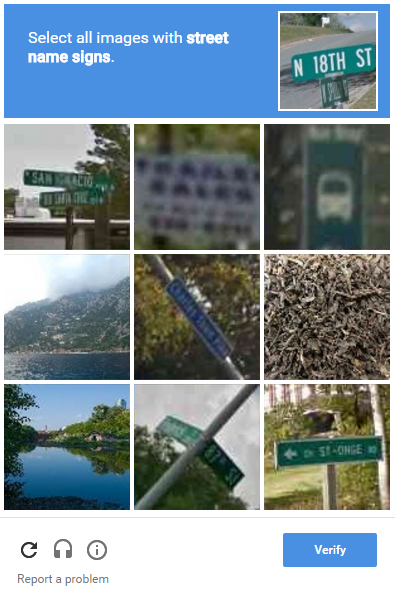
\includegraphics[width=0.3\textwidth]{Graphics/Screenshots/recaptchaFill}}}
				\caption{Recaptcha prompt.}
				\label{fig:recaptcha1}
			\end{figure}
			\item If the recaptcha security check is successful the checkbox will look like figure \ref{fig:recaptcha2}.
			\begin{figure}[H]
				\centerline{\fbox{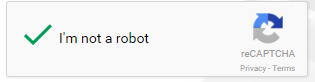
\includegraphics[width=0.3\textwidth]{Graphics/Screenshots/recaptchaCorrect}}}
				\caption{Passed recaptcha security check.}
				\label{fig:recaptcha2}
			\end{figure}
			\item The user will now be able to click the login button to redirect them to their MyPimsSpace page.
		\end{enumerate}
		\begin{figure}[H]
			\fbox{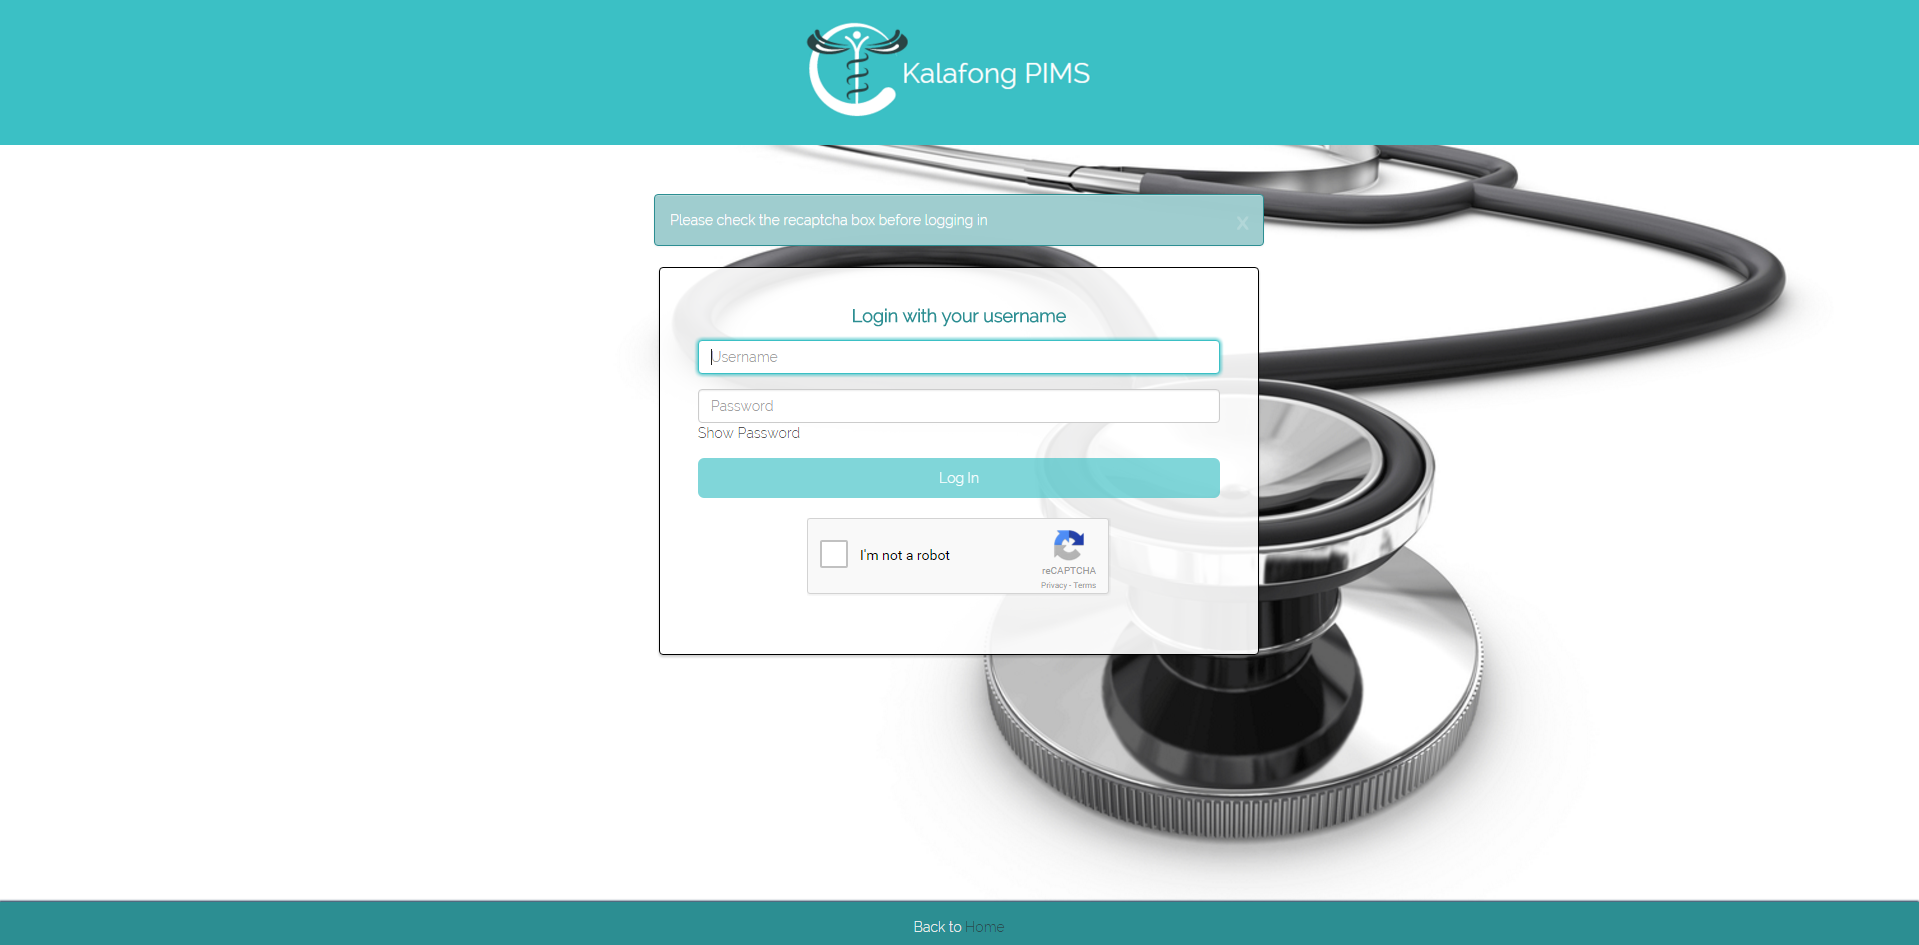
\includegraphics[width=0.5\textwidth]{Graphics/Screenshots/loginI}}
			\fbox{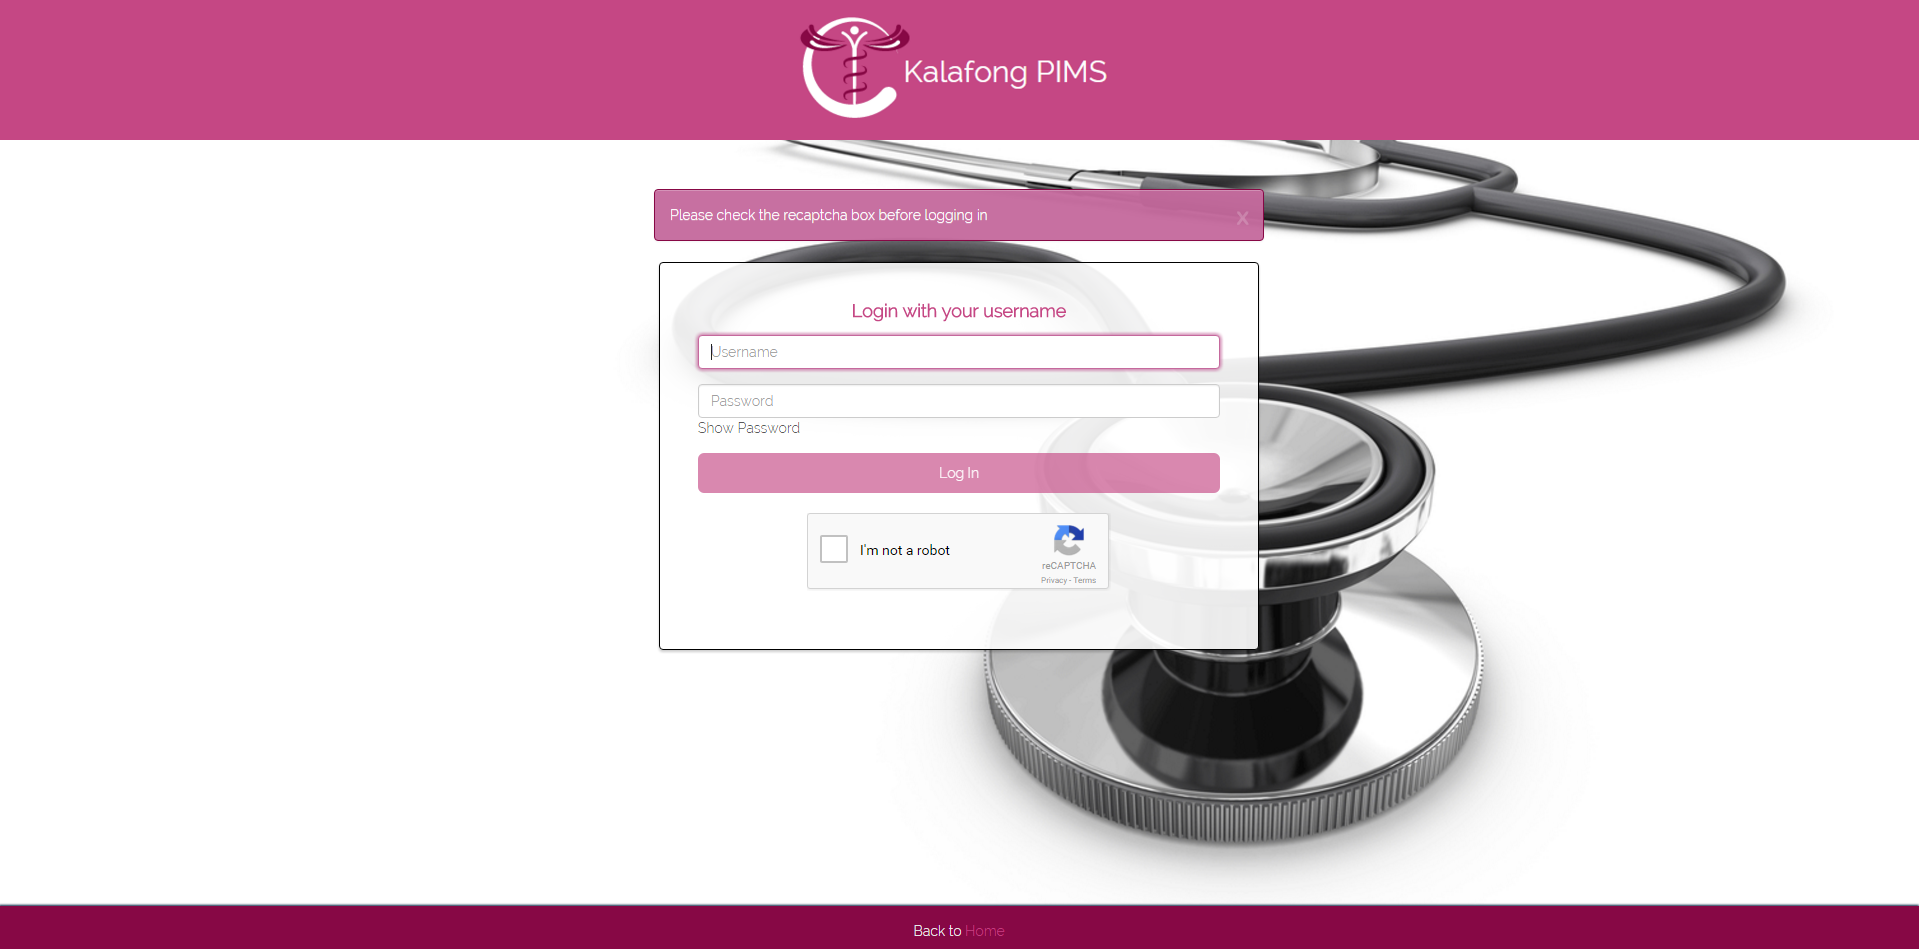
\includegraphics[width=0.5\textwidth]{Graphics/Screenshots/loginR}}
			\caption{Other themed login pages.}
			\label{fig:login2}
		\end{figure}
\newpage
\subsection{Admin Navbar}
	\begin{figure}[H]
		\fbox{
\includegraphics[width=1.0\textwidth]{Graphics/Screenshots/navbar}}
		\caption{The Admin Navbar.}
		\label{fig:navbar1}
	\end{figure}
	\subsubsection{Description} This is the navbar that administrative users will use to help them navigate through pages with ease. A more detailed description can be found below.
	\subsubsection{Detailed Component Description}
		\begin{enumerate}
			\item \textbf{Logo:} This is the logo for the Kalafong PIMS and if clicked will link the user back to their MyPimsSpace page.
			\item \textbf{Active tab:} This is the active tab and will identify to user the current page that are on using a dark blue line at the bottom of its tab. If clicked it will reload the current page. (NOTE: If tab has sub-tabs it will behave as a Submenu tab).
			\item \textbf{Submenu tab:} This is a submenu tab and when clicked will reveal sub tabs that relate to the sub menu tab.
			\item \textbf{Subtab:} Behave like regular tabs but do not underline when active, instead the Submenutab will be underlined.
			\item \textbf{Dropdown tab: } This is a dropdown tab and when click will display a dropdown menu much the like the one in figure \ref{fig:navbar1}.
			\item \textbf{Regular tab: } These tabs will link a user to the specified section. E.g. Predict will link the user to the prediction page.
			\item \textbf{Settings tab:} This tab works similar to a submenu tab and can show all the optional settings for the specific user.
			\item \textbf{Logout tab:} This tab is a regular tab but when clicked the user will be logged out and redirected to the splash page.
		\end{enumerate}
	\subsubsection{How to navigate a Subtab}
		\begin{enumerate}
			\item Click on the Submenu tab which will reveal the Subtabs with an animation
			\item Click on the subtab which is relevant to the page the user would like to access. Then the user will then be redirected to that page.
			\begin{figure}[H]
				\centerline{\fbox{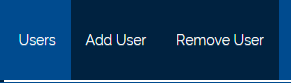
\includegraphics[width=0.4\textwidth]{Graphics/Screenshots/activeNavbar}}}
				\caption{Submenu tab with subtabs visible}
				\label{fig:navbar2}
			\end{figure}
		\end{enumerate}
	\subsubsection{How to navigate a dropdown menu}
		\begin{enumerate}
			\item Click on the Submenu tab which will reveal the dropdown menu.
			\item Click on the dropdown tab which is relevant to the page the user would like to access. Then the user will then be redirected to that page.
			\begin{figure}[H]
				\centerline{\fbox{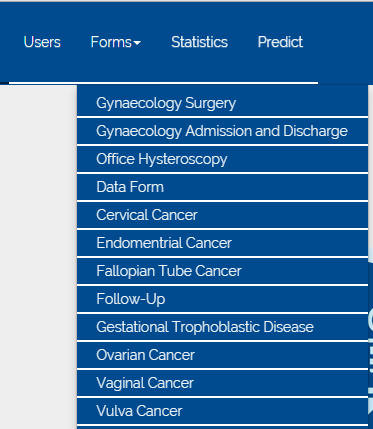
\includegraphics[width=0.4\textwidth]{Graphics/Screenshots/navbarDropdown}}}
				\caption{Dropdown menu}
				\label{fig:navbar3}
			\end{figure}
		\end{enumerate}
	\subsubsection{How to navigate a regular tab}
		\begin{enumerate}
			\item Click on the regular tab which is relevant to the page the user would like to access. Then the user will then be redirected to that page.
		\end{enumerate}
	\subsubsection{How to navigate the settings tab}
		\begin{enumerate}
			\item Click on the Settings tab which will reveal the Subtabs with an animation
			\item Click on the subtab which is relevant to the page the user would like to access. Then the user will then be redirected to that page.
			\begin{figure}[H]
				\centerline{\fbox{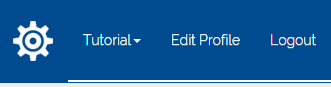
\includegraphics[width=0.4\textwidth]{Graphics/Screenshots/activeSettings}}}
				\caption{Active settings menu}
				\label{fig:navbar3}
			\end{figure}
		\end{enumerate}
	\subsubsection{How to Logout}
		\begin{enumerate}
			\item Click the logout tab and the user will be logged out.
		\end{enumerate}
\subsection {Regular User Navbar}
	\begin{figure}[H]
		\fbox{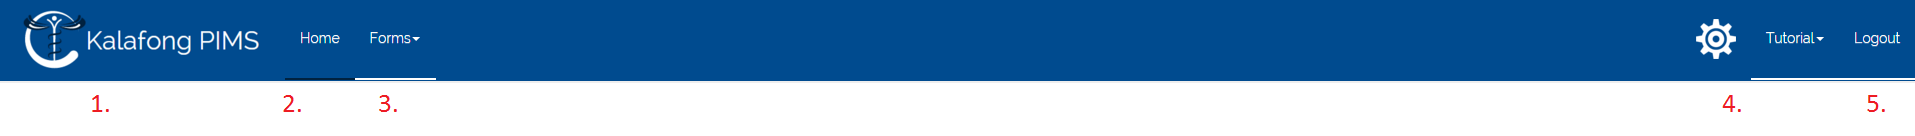
\includegraphics[width=1.0\textwidth]{Graphics/Screenshots/navbarUser}}
		\caption{The User Navbar.}
		\label{fig:navbar4}
	\end{figure}
	\subsubsection{Description} This is the navbar that users will use to help them navigate through pages with ease. A more detailed description can be found below.
	\subsubsection{Detailed Component Description}
		\begin{enumerate}
			\item \textbf{Logo:} This is the logo for the Kalafong PIMS and if clicked will link the user back to their MyPimsSpace page.
			\item \textbf{Active tab:} This is the active tab and will identify to user the current page that are on using a dark blue line at the bottom of its tab. If clicked it will reload the current page. (NOTE: If tab has sub-tabs it will behave as a Submenu tab).
			\item \textbf{Dropdown tab: } This is a dropdown tab and when click will display a dropdown menu much the like the one in figure \ref{fig:navbar1}.
			\item \textbf{Settings tab:} This is a settings tab and when clicked will reveal sub tabs that relate to the sub menu tab.
			\item \textbf{Logout tab:} This tab is a regular tab but when clicked the user will be logged out and redirected to the splash page.
		\end{enumerate}
	\subsubsection{How to navigate a dropdown menu}
		\begin{enumerate}
			\item Click on the Submenu tab which will reveal the dropdown menu.
			\item Click on the dropdown tab which is relevant to the page the user would like to access. Then the user will then be redirected to that page.
			\begin{figure}[H]
				\centerline{\fbox{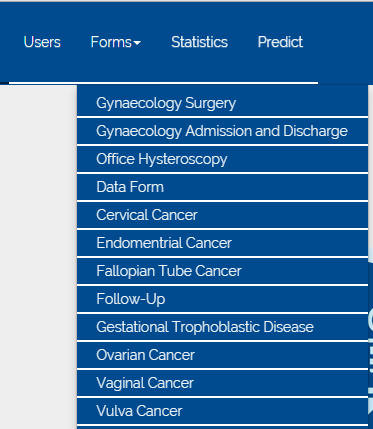
\includegraphics[width=0.4\textwidth]{Graphics/Screenshots/navbarDropdown}}}
				\caption{Dropdown menu}
				\label{fig:navbar5}
			\end{figure}
		\end{enumerate}
	\subsubsection{How to navigate a regular tab}
		\begin{enumerate}
			\item Click on the regular tab which is relevant to the page the user would like to access. Then the user will then be redirected to that page.
		\end{enumerate}
	\subsubsection{How to navigate the settings tab}
		\begin{enumerate}
			\item Click on the Settings tab which will reveal the Subtabs with an animation
			\item Click on the subtab which is relevant to the page the user would like to access. Then the user will then be redirected to that page.
			\begin{figure}[H]
				\centerline{\fbox{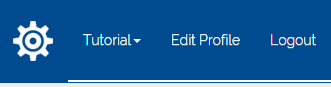
\includegraphics[width=0.4\textwidth]{Graphics/Screenshots/activeSettings}}}
				\caption{Settings menu. NOTE: This is the admin's settings menu and edit profile is not included in the regular users setting's subtabs.}
				\label{fig:navbar6}
			\end{figure}
		\end{enumerate}
	\subsubsection{How to Logout}
		\begin{enumerate}
			\item Click the logout tab and the user will be logged out.
		\end{enumerate}
\subsection{Home Icons}
	\begin{figure}[H]
		\fbox{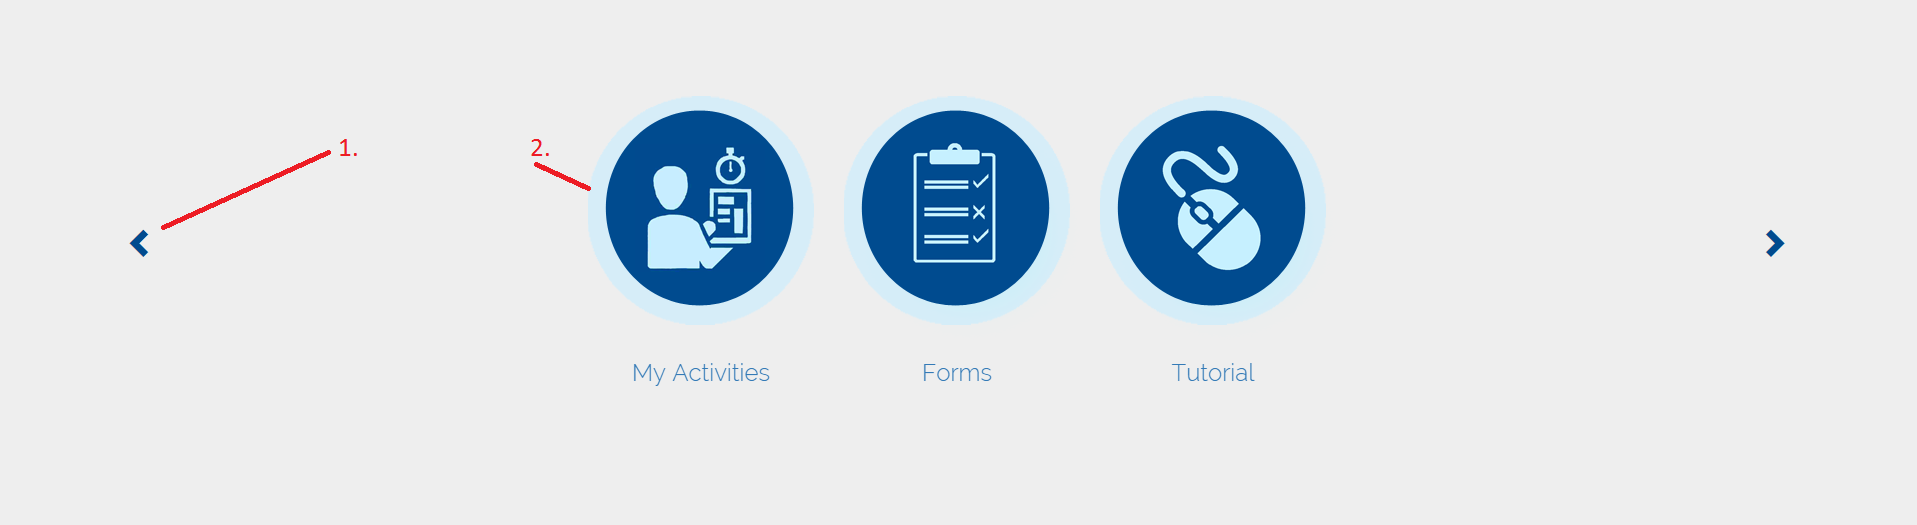
\includegraphics[width=1.0\textwidth]{Graphics/Screenshots/icons}}
		\caption{Admin \& User Home Icons}
		\label{fig:icons1}
	\end{figure}
	\begin{figure}[H]
		\fbox{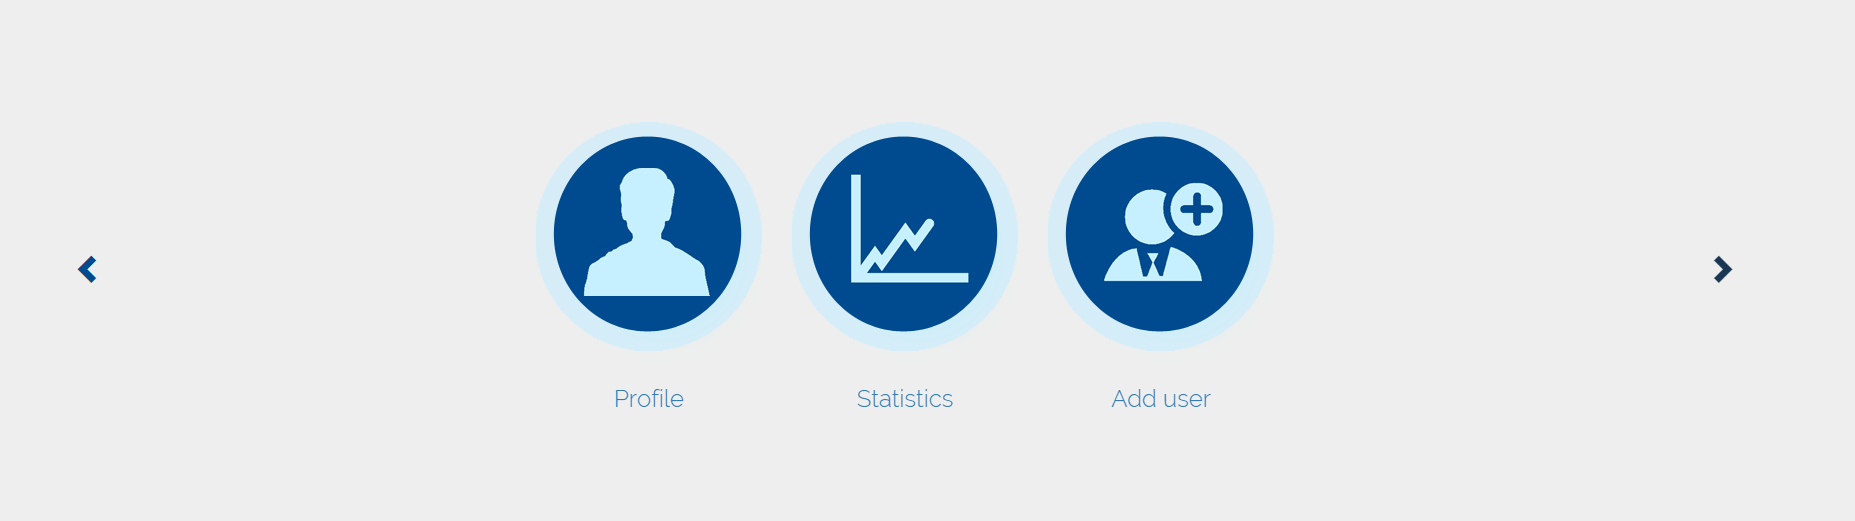
\includegraphics[width=1.0\textwidth]{Graphics/Screenshots/icons2}}
		\caption{More Admin Home Icons}
		\label{fig:icons2}
	\end{figure}
	\subsubsection{Description} The home icons are put in place to ease up usability for users as well as provide an aesthetically pleasing way of navigating the web application. The animation in place is more aesthetic for a regular user as they have limited icons and thus can only navigate through the same set of icons.
	\subsubsection{Detailed Component Description}
		\begin{enumerate}
			\item \textbf{Navigation Arrow:} This arrow is used to navigate through the home icons.
			\item \textbf{Home icon:} This is used as a point of navigation, home icons can either be links or have a submenu links.
		\end{enumerate}
	\subsubsection{How to navigate home icons}
		\begin{enumerate}
			\item By clicking the on the navigations arrows
		\end{enumerate}
		\begin{center} OR \end{center}
		\begin{enumerate}
			\item By clicking the left and right keyboard arrows
		\end{enumerate}
	\subsubsection{How to access icons with submenus}
		\begin{enumerate}
			\item Click on a home icon with a submenu(Tutorial, Statistics(Admin Only), Forms, Activity)
			\item Click on the link that navigates to the desired page.
		\end{enumerate}



\section{Using the System}
\subsection{Fill Forms}
	\begin{figure}[H]
		\centerline{\fbox{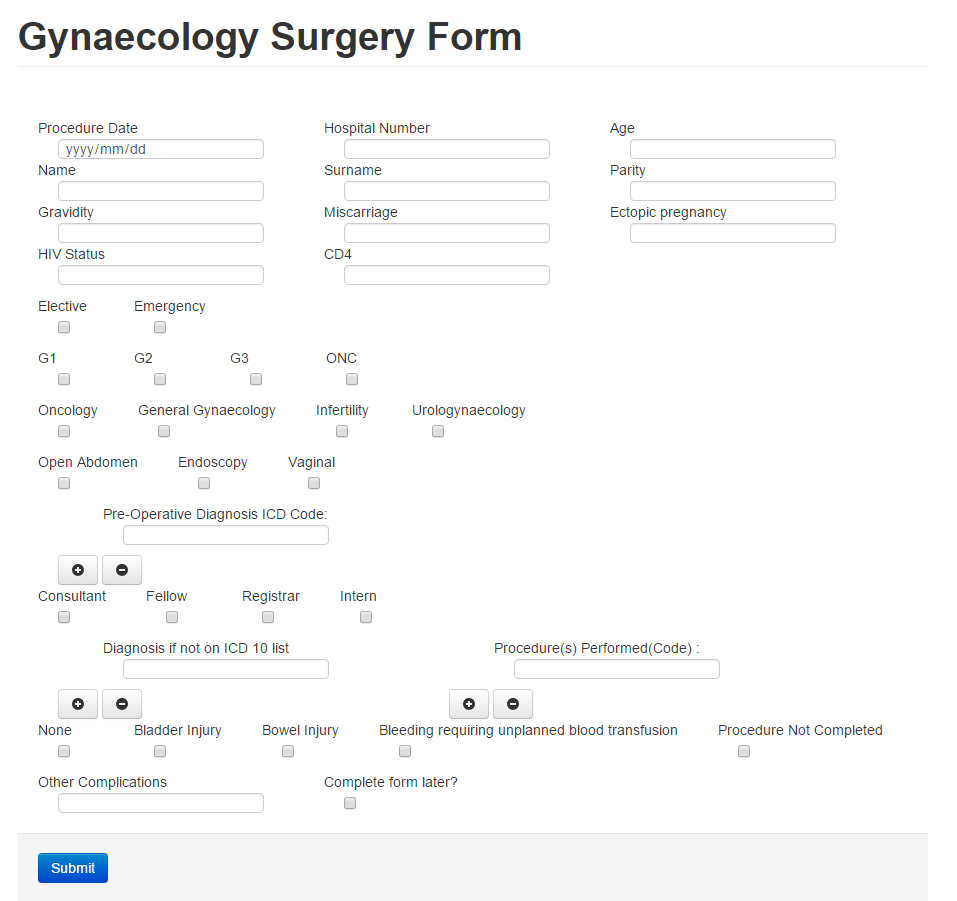
\includegraphics[width=0.8\textwidth]{Graphics/Screenshots/fillForms}}}
		\caption{An example of a form}
		\label{fig:forms1}
	\end{figure}
	\subsubsection{Description} This section is where users can input data into the hospital forms for the system. 
	\subsubsection{Detailed Component Description}
		\begin{enumerate}
			\item \textbf{Input box:} This is an input field where users will place the required information needed for that field.
			\item \textbf{Check box:} This is check box in which users can check if the data collected meets the required checkbox.
			\item \textbf{ICD 10 input box:} This is an input box where users will place the required information needed for that field. Unlike regular input boxes these input boxes allow users to add and remove boxes using the + and - icons.
			\item \textbf{Submit button:} Users can click this button to submit the button once all information has been completed.
		\end{enumerate}
	\subsubsection{How to fill forms}
		\begin{enumerate}
			\item Fill in all required information in all the input boxes and check boxes.
			\item Click on the submit button.
		\end{enumerate}
	\subsubsection{How to fill in ICD 10 Codes}
		\begin{enumerate}
			\item NOTE: To help in ICD codes there is an added usability navbar to provide users with ICD 10 codes. This simplifies filling in information. Relevant sections can be clicked on and a dropdown list will be shown. Examples of the navbar and the dropdown can be found below.
			\begin{figure}[H]
				\centerline{\fbox{
\includegraphics[width=1.0\textwidth]{Graphics/Screenshots/formsHelper}}}
				\caption{ICD 10 Codes navbar.}
				\label{fig:forms2}
			\end{figure}
			\begin{figure}[H]
				\centerline{\fbox{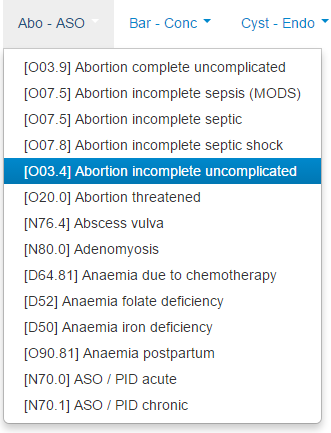
\includegraphics[width=0.3\textwidth]{Graphics/Screenshots/formsHelperDropdown}}}
				\caption{ICD 10 Codes Dropdown.}
				\label{fig:forms3}
			\end{figure}
			\item Fill in relevant ICD code into the input box
			\item Add extra field if more codes are needed.
			\item Repeat 1 and 2 as much as needed.
		\end{enumerate}
\subsection{Statistics Queries}
	\begin{figure}[H]
		\centerline{\fbox{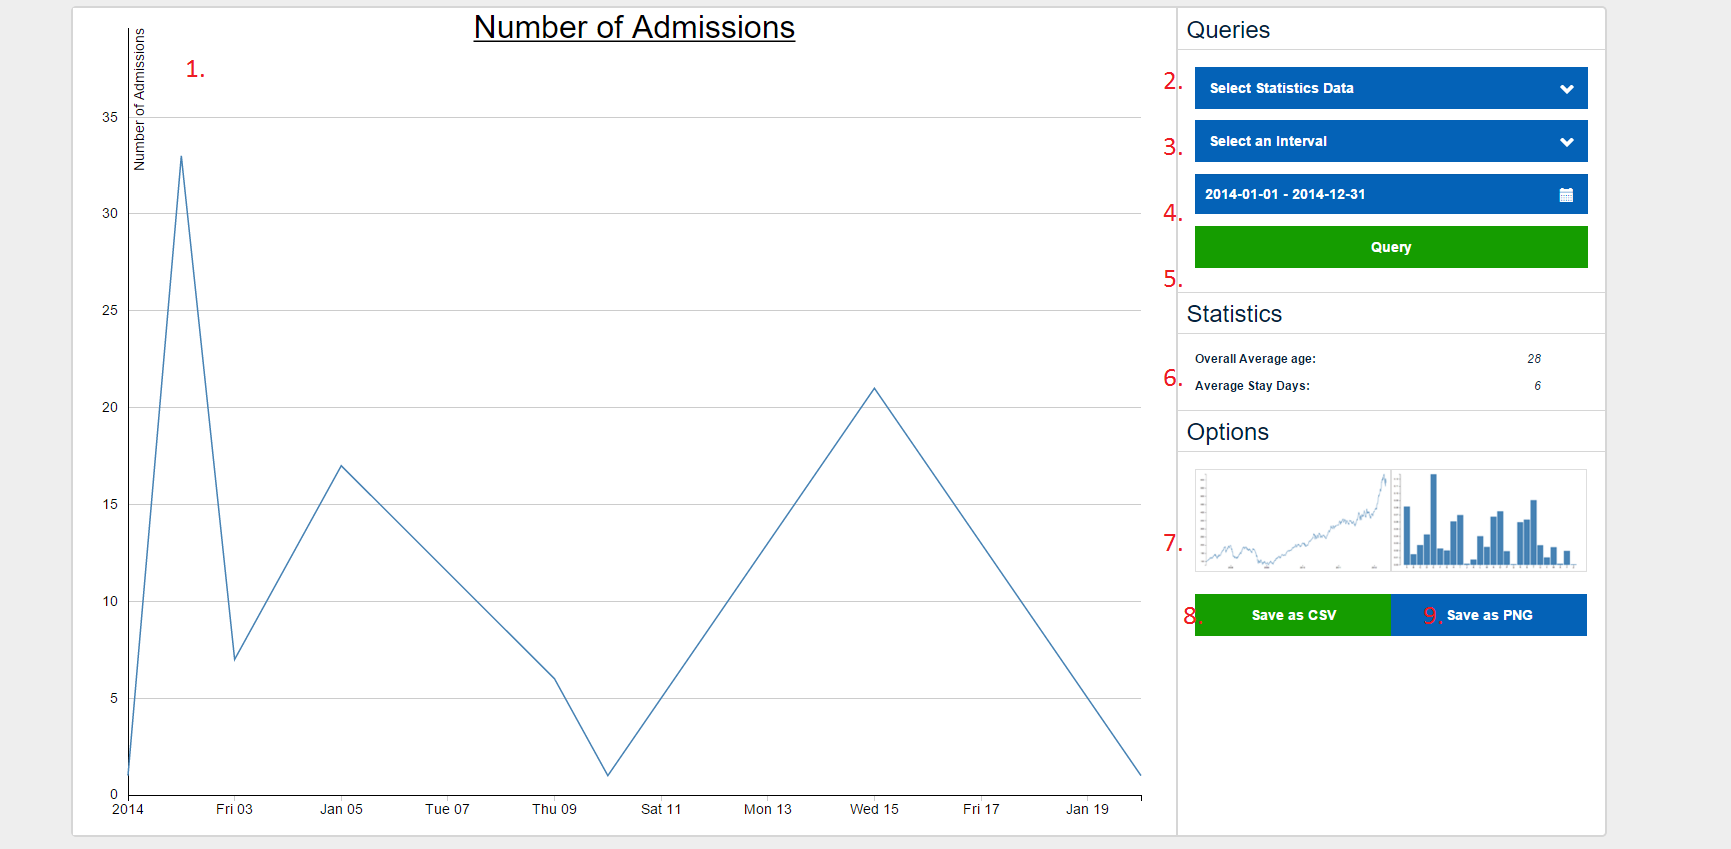
\includegraphics[width=1.0\textwidth]{Graphics/Screenshots/statsQuery}}}
		\caption{Statistical Queries Page.}
		\label{fig:statsQ1}
	\end{figure}
	\subsubsection{Description} This page allows the administrative user to query statistics to obtain information for research purposes.
	\subsubsection{Detailed Component Description}
		\begin{enumerate}
			\item \textbf{Statistics Graph:} This is the graph that represents the statistics data queried. The default graph show upon page load is always the number of admissions over a daily interval. 
			\item \textbf{Statistics Data Dropdown List:} This is a dropdown list that allows the user to select the data they would like to query.
			\item \textbf{Interval Dropdown List:} This is a dropdown list that allows the user to select the interval they would like the data to be grouped by.
			\item \textbf{Date Selector:} This is a selection input box that allows the user to choose the period in which they want the data from. E.g. They would choose a start date of 01/01/2014 up until an end date of 31/10/2014.
			\item \textbf{Query Button:} This button can be clicked to create a new statistics graph with options selected by user.
			\item \textbf{Statistics Average Section:} This section contains averages for certain statistics collected.
			\item \textbf{Graph Type Selector: } This is two selectors that allow the user to choose whether the information is showed as a bar graph or a line graph.
			\item \textbf{Save as CSV:} This allows the user to save the data represented into a CSV file.
			\item \textbf{Save as PNG:} This allows the user to save the data represented as a PNG image file.
		\end{enumerate}
	\subsubsection{How to query statistics:}
		\begin{enumerate}
			\item Select the statistics data from the statistics data dropdown list. An example of the dropdown list in use is shown in figure \ref{fig:statsQ2}.
			\begin{figure}[H]
				\centerline{\fbox{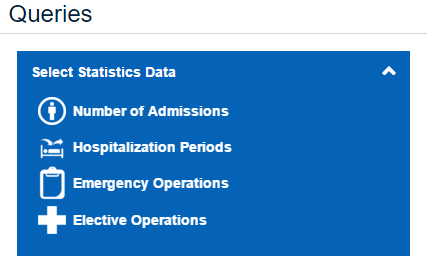
\includegraphics[width=0.4\textwidth]{Graphics/Screenshots/statisticsData}}}
				\caption{Statistics Data Dropdown List in use.}
				\label{fig:statsQ2}
			\end{figure}
			\item Select the interval period from the interval dropdown list. An example of the dropdown list in use is show in figure \ref{fig:statsQ3}.
			\begin{figure}[H]
				\centerline{\fbox{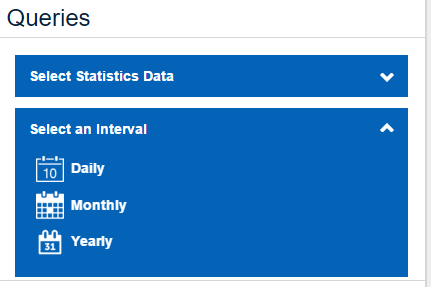
\includegraphics[width=0.4\textwidth]{Graphics/Screenshots/intervalData}}}
				\caption{Interval Dropdown List in use.}
				\label{fig:statsQ3}
			\end{figure}
			\item Select the start and end dates from the Date Selector(Always start with the start date). An example of start and end dates selected is shown in figure \ref{fig:statsQ4}
			\begin{figure}[H]
				\centerline{\fbox{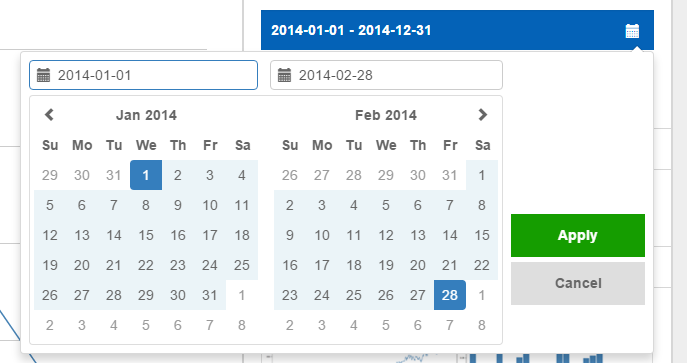
\includegraphics[width=0.4\textwidth]{Graphics/Screenshots/dateSelection}}}
				\caption{Statistics Data Dropdown List in use.}
				\label{fig:statsQ4}
			\end{figure}
			\item Click on the query button and the new graph with the options selected will be shown.
		\end{enumerate}
	\subsubsection{How to select the graph type}
		\begin{enumerate}
			\item Choose either the bar or line graph from the Graph type selector
		\end{enumerate}
	\subsubsection{How to save graph as CSV}
		\begin{enumerate}
			\item Click on the save as CSV button.
		\end{enumerate}
	\subsubsection{How to save graph as PNG}
		\begin{enumerate}
			\item Click on the save as PNG button.
		\end{enumerate}
	\subsubsection{How to select the graph type}
		\begin{enumerate}
			\item Choose either the bar or line graph from the Graph type selector
		\end{enumerate}
	\subsubsection{How the graphs are created:}
		\begin{enumerate}
			\item Initially the system will obtain the data based off the options select by the user in their query(See how to query statistics). It will send the information obtained in a JSON format and the system will determine what statistics will be needed to sent back to page. These requests and responses are all done on the same page through the use of AJAX.
			\item Once the system has determined what needs to send back by querying the mongo database use an aggregate function, it will respond back using JSON formatted object.
			\item The client side will then receive this information and sent it to a local javascript function that creates the graph
			\item Initially the graph sets the margins. The margins of graph are created by working out the margins on the page based off of the screens resolution.
			\item The data is then analysed to scale the x and y axes correctly.
			\item The data is then finally passed into the graph and then the line or bar graphs are drawn.
		\end{enumerate}
\subsection{Statistics Dashboard}
	\begin{figure}[H]
		\centerline{\fbox{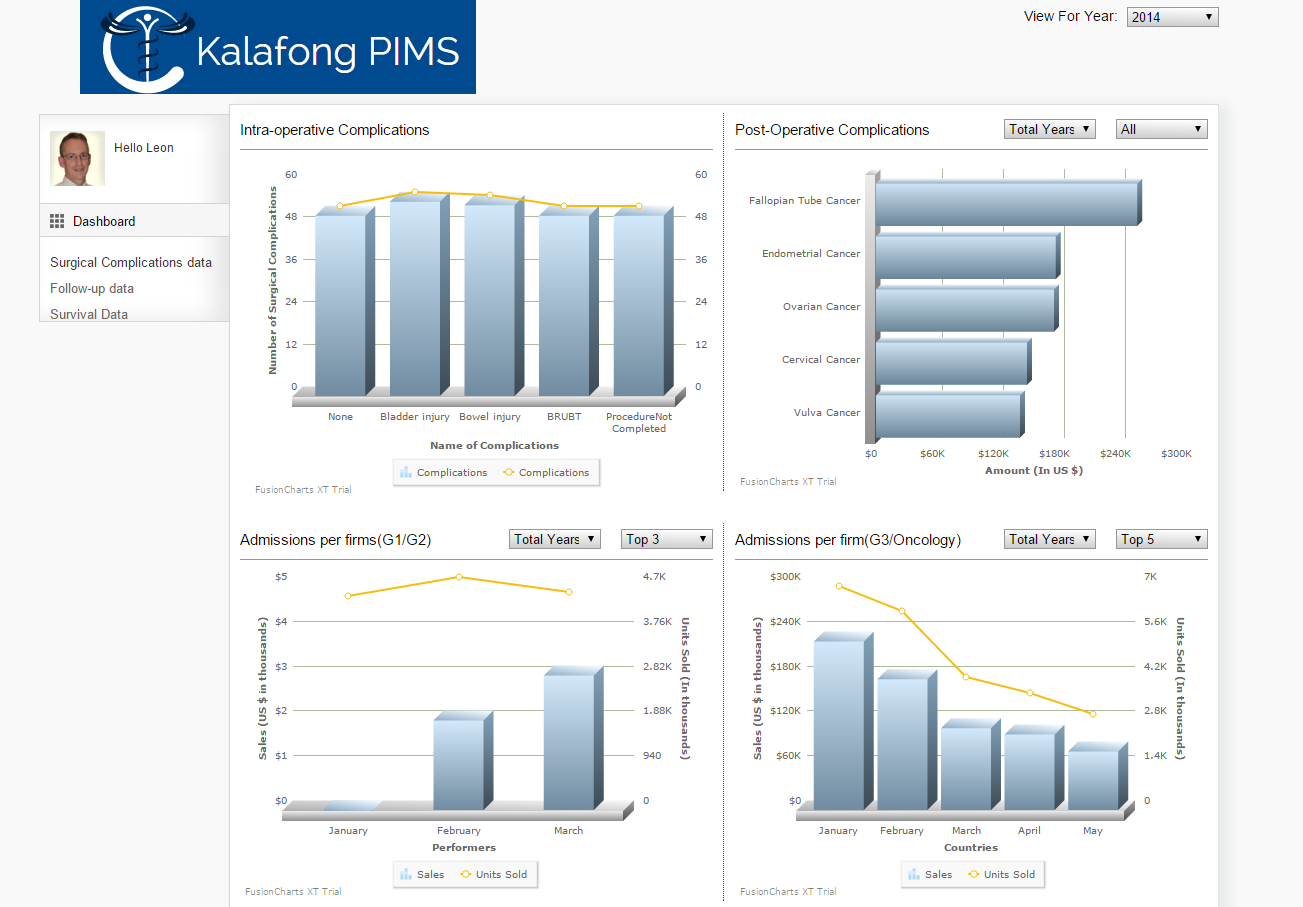
\includegraphics[width=1.0\textwidth]{Graphics/Screenshots/dashboard}}}
		\caption{The Statistics Dashboard.}
		\label{fig:dash1}
	\end{figure}
	\subsubsection{Description} This dashboard is available to the admin user and allows them to an overall summary of multiple graphs.
	\subsubsection{Detailed Component Description}
		\begin{enumerate}
			\item \textbf{Dashboard Sections:} This section of the dashboard allows the user to view graphs grouped into their respective sections. 
			\item \textbf{Graph:} This is a graph that represents certain data.
			\item \textbf{Year selector: } This allows the user to select what year the graphs data represents.
			\item \textbf{Total Years Selector: } This allows the user to select the years for that specific graph.
			\item \textbf{Top Selector:} This allows the user to choose whether the graph shows the Top 5 statistics or all of them.
		\end{enumerate}
	\subsubsection{How to select the top 5 of a specific graph.}
		\begin{enumerate}
			\item Click on the top selector and choose the top 5 from the dropdown list.
		\end{enumerate}
	\subsubsection{How the graphs are created in the dasboard}
		\begin{enumerate}
			\item On intitial page load, there are multiple ajax requests that post to specific server scripts.
			\item These server scripts willl calll functions that will query the database using aggregation and/or count functions.
			\item Once the data is obtained from the database the functions will respond back to their original ajax callees with arrays.
			\item Upon AJAX success they will take these arrays and call the draw graph functions.
		\end{enumerate}
\subsection{Add User}
	\begin{figure}[H]
		\centerline{\fbox{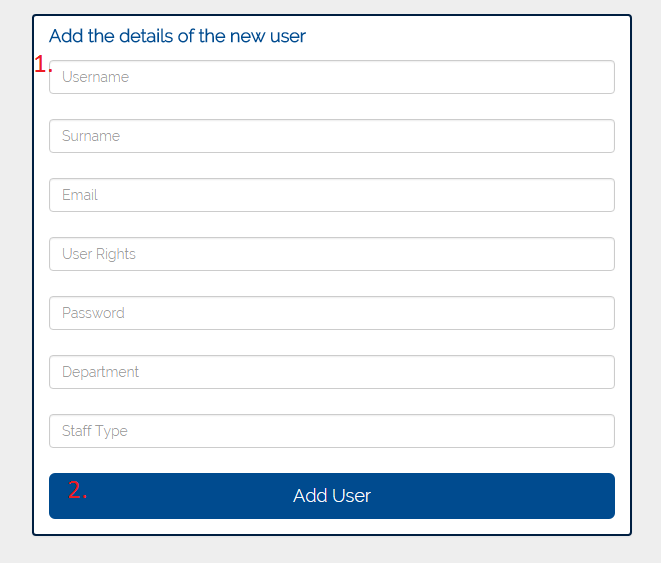
\includegraphics[width=0.8\textwidth]{Graphics/Screenshots/addUser}}}
		\caption{The Add User Box}
		\label{fig:addUser}
	\end{figure}
	\subsubsection{Description} This is the add user input box which allows the admin user to add users that can log into the system and perform certain responsibilities.
	\subsubsection{Detailed Component Description}
		\begin{enumerate}
			\item \textbf{Input box:} This is an input box in which the user can fill the necessary information in the box.
			\item \textbf{Add User Button:} This button when clicked will take all the information from the form and use it to add a user to the system.
		\end{enumerate}
	\subsubsection{How to add a user}
		\begin{enumerate}
			\item Fill in the user's name
			\item Fill in the user's surname
			\item Fill in the user's email(must be valid)
			\item Fill in the user's rights (1 for admin, 0 for regular user)
			\item Fill in the user's password
			\item Fill in the user's department (Must be a valid department)
			\item Fill in the user's staff type (Must be a valid staff type)
		\end{enumerate}
	\subsubsection{How add user works}
		\begin{enumerate}
			\item Initially the program will post all the values in object format to the server. 
			\item These values willl be validated. Iif the values are invalid,  an error will be sent through a response and the client side will generate an appropriate error message.
			\item Upon successful validation the system will insert all values into the database through a simple insert function.
			\item Then respond with a message stating whether the user was successfully added or not.
		\end{enumerate}
\subsection{Remove User}
	\begin{figure}[H]
		\centerline{\fbox{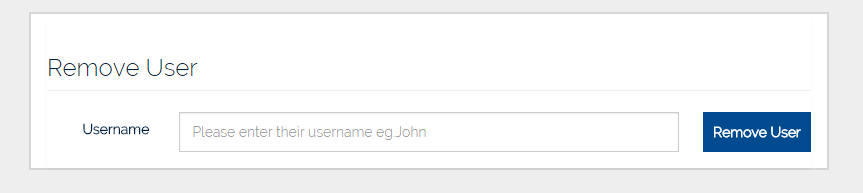
\includegraphics[width=0.8\textwidth]{Graphics/Screenshots/removeUser}}}
		\caption{The Remover User Form.}
		\label{fig:removeUser1}
	\end{figure}
	\subsubsection{Description} This section allows an admin user to remove a user from the system.
	\subsubsection{Detailed Component Description}
		\begin{enumerate}
			\item \textbf{Username input box:} This input box is where the admin user specifies the username of the user to be removed from the system.
			\item \textbf{Remove user button:} This button when clicked the username specified is valid will remove the user from the database.
		\end{enumerate}
	\subsubsection{How to remove a user}
		\begin{enumerate}
			\item Fill in a valid user name in the username input box.
			\item Click on the remove user button.
		\end{enumerate}
\subsection{Update Profile}
	\begin{figure}[H]
		\centerline{\fbox{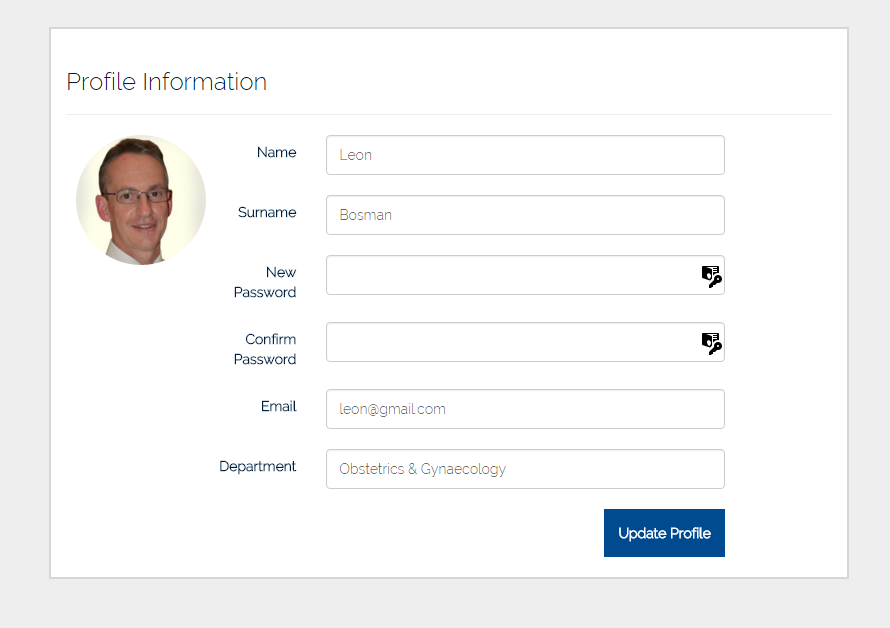
\includegraphics[width=0.8\textwidth]{Graphics/Screenshots/profileInformation}}}
		\caption{The Update Profile Page}
		\label{fig:updateProf1}
	\end{figure}
	\subsubsection{Description} 
	\subsubsection{Detailed Component Description}
		\begin{enumerate}
			\item \textbf{Username input box:} This input box is where the admin user specifies the username of the user to be removed from the system.
			\item \textbf{Update profile button:} This is a button that when clicked will update all the relevant information for the user.
		\end{enumerate}
	\subsubsection{How to update your profile}
		\begin{enumerate}
			\item User must fill in fields that need to be updated.
			\item User must click on the update profile button.
		\end{enumerate}
\subsection{Predict}
	\begin{figure}[H]
		\centerline{\fbox{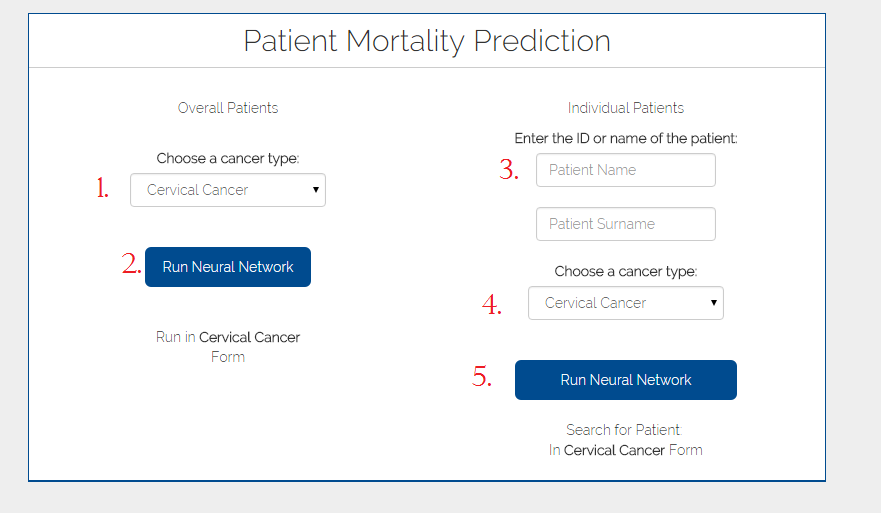
\includegraphics[width=1.0\textwidth]{Graphics/Screenshots/predict}}}
		\caption{The Prediction Page.}
		\label{fig:predict1}
	\end{figure}
	\subsubsection{Description} This page predicts the mortality of a patient using artificial intelligence. The artificial intelligence analyses the statistics and determines the likelihood of whether the patient will survive the cancer.
	\subsubsection{Detailed Component Description}
		\begin{enumerate}
			\item \textbf{Overall Patient Cancer Dropdown list:} This is a dropdown list of all the cancer types.
			\item \textbf{Overall Patient Neural Network Button:} This is the button that runs the overall patients neural network.
			\item \textbf{Individual Patient Cancer Input box}: This is an input box for individual patients.
			\item \textbf{Individual Patient Cancer Dropdown list:} This is a dropdown list of all the cancer types.
			\item \textbf{Individual Patient Cancer Neural Network button:} This is the button that runs the individual patients neural network.
		\end{enumerate}
	\subsubsection{How to predict the mortality rate of patients overall}
		\begin{enumerate}
			\item Select the cancer type from the overall patient cancer dropdown list
			\item Click the overall patient neural network button. NOTE: The end result should be similar to figure \ref{fig:predict2}
			\begin{figure}[H]
				\centerline{\fbox{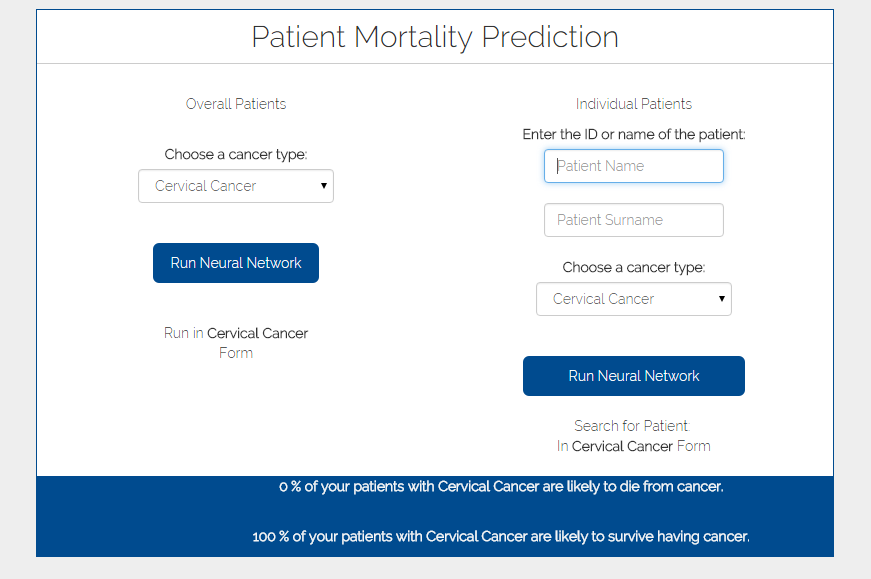
\includegraphics[width=1.0\textwidth]{Graphics/Screenshots/predicted}}}
				\caption{The prediction page after being run.}
				\label{fig:predict2}
			\end{figure}
		\end{enumerate}
	\subsubsection{How to predict the mortality rate of a patient based on the individual patients symptoms.}
		\begin{enumerate}
			\item Fill in the patients Username or ID and their surname in the individual patient cancer input boxes.
			\item Select the cancer type from the individual patient cancer dropdown list
			\item Click the individual patient cancer neural network button. NOTE: The end result should look similar to figure \ref{fig:predict2}
		\end{enumerate}
\subsection{Tutorial} 
	\begin{figure}[H]
		\centerline{\fbox{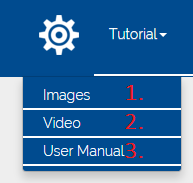
\includegraphics[width=0.3\textwidth]{Graphics/Screenshots/tutorialDropdown}}}
		\caption{The tutorial dropdown menu}
		\label{fig:tut1}
	\end{figure}
	\begin{figure}[H]
		\centerline{\fbox{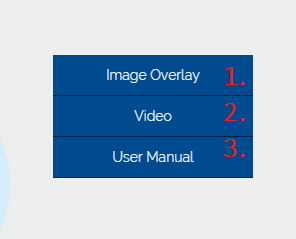
\includegraphics[width=0.3\textwidth]{Graphics/Screenshots/tutorialIcon}}}
		\caption{The tutorial icon menu}
		\label{fig:tut2}
	\end{figure}
	\subsubsection{Description}This section describes how a user can access the different tutorials through the web application.
	\subsubsection{Detailed Component Description}
		\begin{enumerate}
			\item \textbf{Image Overlay Link:} This is a link that loads the image tutorial overlay.
			\item \textbf{Video Link:} This is a link the user to video tutorial.
			\item \textbf{User Manual Link:} This link downloads the user manual in pdf form.
		\end{enumerate}
	\subsubsection{How to access the image overlay tutorial}
		\begin{enumerate}
			\item If user is on the my pims space page. Click on the tutorial Icon.
			\item Select the image overlay link.
		\end{enumerate}
		\begin{center}OR\end{center}
		\begin{enumerate}
			\item Click on the settings icon in the navbar.
			\item Click on the tutorial dropdown
			\item Select the images link
		\end{enumerate}
	\subsubsection{How to access the video tutorial}
		\begin{enumerate}
			\item If user is on the my pims space page. Click on the tutorial Icon.
			\item Select the Video link.
		\end{enumerate}
		\begin{center}OR\end{center}
		\begin{enumerate}
			\item Click on the settings icon in the navbar.
			\item Click on the tutorial dropdown
			\item Select the video link
		\end{enumerate}
	\subsubsection{How to download the user manual}
		\begin{enumerate}
			\item If user is on the my pims space page. Click on the tutorial Icon.
			\item Select the user manual link.
		\end{enumerate}
		\begin{center}OR\end{center}
		\begin{enumerate}
			\item Click on the settings icon in the navbar.
			\item Click on the tutorial dropdown
			\item Select the user manual link
		\end{enumerate}
\newpage





\section{Troubleshooting}
\subsection{Introduction}
This section contains a series of tables that describe
possible solutions to problems that may occur when
using your PC. Each table contains: \\
\begin{itemize}
	\item Symptoms that describe the sign or warning message for the type of problem.
	\item Possible solutions that describe what you should
do to try to solve the problem. 
\end{itemize}

\setlength{\arrayrulewidth}{1mm}
\setlength{\tabcolsep}{18pt}
\renewcommand{\arraystretch}{1.5}
 

\begin{tabular}{ |p{3.5cm}|p{3.5cm} | p{3.5cm}|  }
\hline
\multicolumn{3}{|c|}{Troubleshooting} \\
\hline
Symptoms & Possible solution  & Graphical Errors\\
\hline
You press the login button and nothing happens & 1. You entered the wrong username/password combination. 1.1 Click show password to see what you have typed. 1.2 Recheck your email from admin to ensure you are using the correct username/password combination. 1.3 You have not clicked the recaptcha box.   & Refer to Troubleshooting figure 1\\ \hline
Cannot add new user & 2. You have to fill all the textboxes & Refer to Troubleshooting figure 1\\ \hline
Cannot edit profile    &Make sure you have internet connection & Refer to Troubleshooting figure 1 \\ \hline
Cannot query statistics & Make sure you have selected an option for each dropdownlist. Ensure you have clicked the query button.  & Refer to Troubleshooting figure 1\\
\hline
\end{tabular}

\subsection{Troubleshooting figures}
Use these images in reference with the troubleshooting table.

\begin{itemize}
	\item Figure 1
	\begin{figure}[H]
        \centerline{\fbox{
\includegraphics[width=0.5\textwidth]{Graphics/Troubleshooting/recapture}}}
		\caption{Content Setting}
      \end{figure}
	\item Figure 2
	
	\item Figure 3
\end{itemize}



\end{document}